\documentclass{plt}

\title{Generating Code and Running Programs}
\author{Stephen A. Edwards}
\institute{Columbia University}
\date{Fall 2018}
\titlegraphic{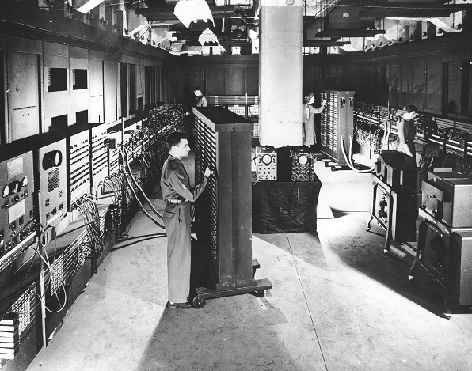
\includegraphics[width=0.4\textwidth]{eniac.jpg}}

\tikzset{
  connecting lines/.style={remember picture, overlay,
    every path/.style={->,red,opacity=0.5,line width=2pt}}
}

%\newcommand{\hlt}[1]{\textcolor{red}{#1}}
\newcommand{\lab}[3]{\tikz{\useasboundingbox (0,0);
    \node [draw, anchor=west, fill=black!10,rectangle callout,
           callout absolute pointer={(1pt,3pt)}] at (#1,#2) {\rmfamily{#3}}; 
}}

\newcommand{\rnode}[2]{\tikz[baseline,remember picture]
  \node [anchor=text,inner sep=0pt] (#1) {#2};}

\newcommand{\framednode}[2]{\tikz[baseline,remember picture]
  \node [anchor=text,draw] (#1) {#2};}

% Work around a tikz bug
\makeatletter
\def\pgf@test{}
\makeatother

\begin{document}

\maketitle

\part{The Compilation Process}
\frame{\partpage}

\newcommand{\phase}[2]{
$\llap{\textrm{#1}}\left\{
\hbox to 10pc{\hfil
\begin{tabular}{c}
#2
\end{tabular}\hfil}
\right.$
}

\newcommand{\transform}[1]{
$\downarrow$\rlap{\hspace{1pc}\textcolor{red}{#1}}
}

\begin{frame}
  \frametitle{A Long K's Journey into Byte$^\dagger$}

\parskip=0pt
\begin{center}
\phase{Compiler front end}{
Source code \\
\transform{Parser/Semantic Analysis} \\
AST \\
}

\phase{Compiler back end}{
\transform{Intermediate code generation} \\
IR \\
\transform{Optimization} \\
Assembly Code \\
}

\phase{Assembler}{
\transform{Assemble} \\
Relocatable Object Code \\
}

\phase{Linker}{
\transform{Link} \\
Executable \\
}

\phase{Loader}{
\transform{Relocate} \\
In-memory image \\
}

\end{center}

{\footnotesize $\dagger$Apologies to O'Neill}

\end{frame}

\begin{frame}
  \frametitlelogo{Compiler Frontends and Backends}{0.3\textwidth}{pantohorse.png}

The front end focuses on \emph{analysis}:

\begin{itemize}
\item Lexical analysis

\item Parsing

\item Static semantic checking

\item AST generation
\end{itemize}

The back end focuses on \emph{synthesis}:

\begin{itemize}
\item Translation of the AST into intermediate code

\item Optimization

\item Generation of assembly code
\end{itemize}

\end{frame}

\begin{frame}[fragile]{Portable Compilers}

Building a compiler a large undertaking; most try to leverage it by
making it portable.

\begin{center}
\begin{tikzpicture}
    \matrix (network)
            [matrix of nodes,
              column 1/.style={anchor=east},
              column 2/.style={anchor=west},
              column sep={8pc,between origins},
              row sep={2pc,between origins}]
            {
              C & x86 \\
              C++ & ARM \\
              Java & MIPS \\
              Go & PPC \\
              Objective C & AVR \\
              FORTRAN & 68000 \\
            };
\only<1>{
  \foreach \a in {1,...,6}{
    \foreach \b in {1,...,6}{
      \draw (network-\a-1.east) -- (network-\b-2.west);
    }
  }
}
  \only<2>{
    \node [anchor=west] at (network) (ir) {IR};
    \foreach \a in {1,...,6}{
        \draw (network-\a-1.east) -- (ir);
        \draw (ir) -- (network-\a-2.west);
    }
  }
  \end{tikzpicture}

\onslide<2>{
$\underbrace{\hspace{9pc}}_{\text{\begin{tabular}{c}Language-specific\\Frontends\end{tabular}}}$
\hspace{1pc}
$\underbrace{\hspace{8pc}}_{\text{\begin{tabular}{c}Processor-specific\\Backends\end{tabular}}}$
}

\end{center}

\end{frame}


\part{Intermediate Representations/Formats}
\frame{\partpage}

\begin{frame}[fragile]
  \frametitle{Stack-Based IR: Java Bytecode}

  \begin{columns}
    \begin{column}{0.45\textwidth}

\begin{java}
int gcd(int a, int b) {
  while (a != b) {
    if (a > b)
      a -= b;
    else
      b -= a;
  }
  return a;
}
\end{java}

\vspace{2pc}

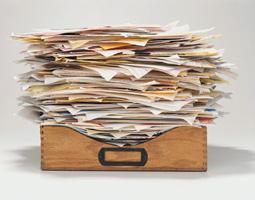
\includegraphics[width=0.75\columnwidth]{stack-of-papers.jpg}
    \end{column}
    \begin{column}{0.55\textwidth}
\fontsize{8}{8}\selectfont
\begin{semiverbatim}
# javap -c Gcd

Method int gcd(int, int)
   0 goto 19

   3 iload_1      \hlt{\textrm{// Push a}}         
   4 iload_2      \hlt{\textrm{// Push b}}
   5 if_icmple 15 \hlt{\textrm{// if a <= b goto 15}}

   8 iload_1      \hlt{\textrm{// Push a}}      
   9 iload_2      \hlt{\textrm{// Push b}}
  10 isub         \hlt{\textrm{// a - b}}
  11 istore_1     \hlt{\textrm{// Store new a}}
  12 goto 19

  15 iload_2      \hlt{\textrm{// Push b}}
  16 iload_1      \hlt{\textrm{// Push a}}  
  17 isub         \hlt{\textrm{// b - a}}
  18 istore_2     \hlt{\textrm{// Store new b}}

  19 iload_1      \hlt{\textrm{// Push a}}
  20 iload_2      \hlt{\textrm{// Push b}}
  21 if_icmpne 3  \hlt{\textrm{// if a != b goto 3}}

  24 iload_1      \hlt{\textrm{// Push a}}
  25 ireturn      \hlt{\textrm{// Return a}}
\end{semiverbatim}
    \end{column}
  \end{columns}

\end{frame}

\begin{frame}
  \frametitlelogo{Stack-Based IRs}{0.3\textwidth}{pancake-stack.jpg}

Advantages:

\begin{itemize}
\item Trivial translation of expressions

\item Trivial interpreters

\item No problems with exhausting registers

\item Often compact
\end{itemize}

Disadvantages:

\begin{itemize}
\item Semantic gap between stack operations and modern register machines

\item Hard to see what communicates with what

\item Difficult representation for optimization
\end{itemize}

\end{frame}

\begin{frame}[fragile]{Register-Based IR: Mach SUIF}

% c2s gcd.c
% do_lower gcd.suif gcd.lsf
% do_s2m gcd.lsf gcd.svm
% do_print gcd.svm

  \begin{columns}
    \begin{column}{0.35\textwidth}
\begin{java}
int gcd(int a, int b) {
  while (a != b) {
    if (a > b)
      a -= b;
    else
      b -= a;
  }
  return a;
}
\end{java}

\vspace{2pc}

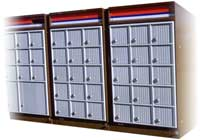
\includegraphics[width=\columnwidth]{mailboxes.jpg}
    \end{column}
    \begin{column}{0.65\textwidth}
\fontsize{8}{8}\selectfont
\begin{semiverbatim}
gcd:
gcd._gcdTmp0:
  sne   $vr1.s32 <- gcd.a,gcd.b
  seq   $vr0.s32 <- $vr1.s32,0
  btrue $vr0.s32,gcd._gcdTmp1  \hlt{\textrm{// if !(a != b) goto Tmp1}}

  sl    $vr3.s32 <- gcd.b,gcd.a
  seq   $vr2.s32 <- $vr3.s32,0
  btrue $vr2.s32,gcd._gcdTmp4  \hlt{\textrm{// if !(a \(<\) b) goto Tmp4}}

  mrk   2, 4   \hlt{\textrm{// Line number 4}}
  sub   $vr4.s32 <- gcd.a,gcd.b
  mov   gcd._gcdTmp2 <- $vr4.s32
  mov   gcd.a <- gcd._gcdTmp2  \hlt{\textrm{// a = a - b}}
  jmp   gcd._gcdTmp5
gcd._gcdTmp4:
  mrk   2, 6
  sub   $vr5.s32 <- gcd.b,gcd.a
  mov   gcd._gcdTmp3 <- $vr5.s32
  mov   gcd.b <- gcd._gcdTmp3  \hlt{\textrm{// b = b - a}}
gcd._gcdTmp5:
  jmp   gcd._gcdTmp0

gcd._gcdTmp1:
  mrk   2, 8
  ret   gcd.a  \hlt{\textrm{// Return a}}
\end{semiverbatim}
    \end{column}
  \end{columns}
\end{frame}

\begin{frame}
  \frametitlelogo{Register-Based IRs}{0.25\textwidth}{cash-register.jpg}

\hlt{\emph{Most common type of IR}}

Advantages:

\begin{itemize}
\item Better representation for register machines

\item Dataflow is usually clear
\end{itemize}

Disadvantages:

\begin{itemize}
\item Slightly harder to synthesize from code

\item Less compact

\item More complicated to interpret
\end{itemize}

\end{frame}

\part{Introduction to Optimization}
\frame{\partpage}

\begin{frame}[fragile]
  \frametitle{Optimization In Action}

\begin{columns}
  \begin{column}[t]{0.4\textwidth}
\mbox{}
\begin{C}
int gcd(int a, int b) {
  while (a != b) {
    if (a < b) b -= a;
    else a -= b;
  }
  return a;
}
\end{C}

\vspace{1pc}

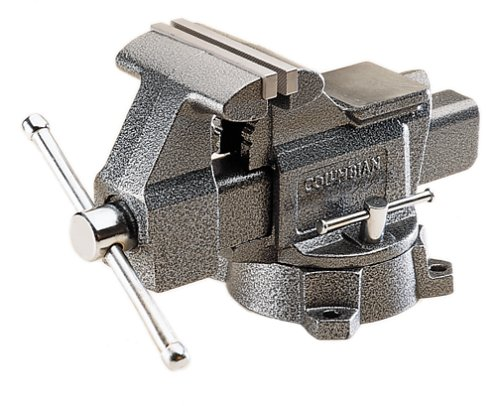
\includegraphics[width=1\columnwidth]{vise.jpg}
  \end{column}
  \begin{column}[t]{0.3\textwidth}
\fontsize{7}{7}\selectfont
\textcolor{red}{GCC on SPARC}
\begin{verbatim}
gcd:  save %sp, -112, %sp
      st   %i0, [%fp+68]
      st   %i1, [%fp+72]
.LL2: ld   [%fp+68], %i1
      ld   [%fp+72], %i0
      cmp  %i1, %i0
      bne  .LL4
      nop 
      b    .LL3
      nop 
.LL4: ld   [%fp+68], %i1
      ld   [%fp+72], %i0
      cmp  %i1, %i0
      bge  .LL5
      nop 
      ld   [%fp+72], %i0
      ld   [%fp+68], %i1
      sub  %i0, %i1, %i0
      st   %i0, [%fp+72]
      b    .LL2
      nop 
.LL5: ld   [%fp+68], %i0
      ld   [%fp+72], %i1
      sub  %i0, %i1, %i0
      st   %i0, [%fp+68]
      b    .LL2
      nop 
.LL3: ld   [%fp+68], %i0
      ret
      restore
\end{verbatim}
  \end{column}
  \begin{column}[t]{0.3\textwidth}
\fontsize{7}{7}\selectfont
\textcolor{red}{GCC -O7 on SPARC}
\begin{verbatim}
gcd:  cmp   %o0, %o1
      be    .LL8
      nop  
.LL9: bge,a .LL2
      sub   %o0, %o1, %o0
      sub   %o1, %o0, %o1
.LL2: cmp   %o0, %o1
      bne   .LL9
      nop
.LL8: retl
      nop
\end{verbatim}
  \end{column}
\end{columns}

\end{frame}

\begin{frame}[fragile]
  \frametitle{Typical Optimizations}

\begin{itemize}

\item Folding constant expressions

1+3 $\rightarrow$ 4

\item Removing dead code

if (0) $\{$ \ldots $\}$ $\rightarrow$ nothing

\item Moving variables from memory to registers

\medskip

\begin{minipage}{0.35\textwidth}
\begin{verbatim}
ld   [%fp+68], %i1
sub  %i0, %i1, %i0
st   %i0, [%fp+72]
\end{verbatim}
\end{minipage}
$\rightarrow$ 
\begin{minipage}{0.4\textwidth}
\begin{verbatim}
sub   %o1, %o0, %o1
\end{verbatim}
\end{minipage}

\medskip

\item Removing unnecessary data movement

\item Filling branch delay slots (Pipelined RISC processors)

\item Common subexpression elimination

\end{itemize}

\end{frame}

\begin{frame}[fragile]
  \frametitle{Machine-Dependent vs.\ -Independent Optimization}

No matter what the machine is, folding constants and eliminating dead
code is always a good idea.

\begin{minipage}{0.35\textwidth}
\begin{verbatim}
a = c + 5 + 3;
if (0 + 3) {
  b = c + 8;
}
\end{verbatim}
\end{minipage}
$\rightarrow$\hspace{1pc}
\begin{minipage}{0.35\textwidth}
\begin{verbatim}
b = a = c + 8;
\end{verbatim}
\end{minipage}

However, many optimizations are processor-specific:

\begin{itemize}
\item Register allocation depends on how many registers the machine has

\item Not all processors have branch delay slots to fill

\item Each processor's pipeline is a little different
\end{itemize}

\end{frame}

\begin{frame}[fragile]{Basic Blocks}

\vbox to 0pt{\vss\hbox to 0.6\textwidth{\hfill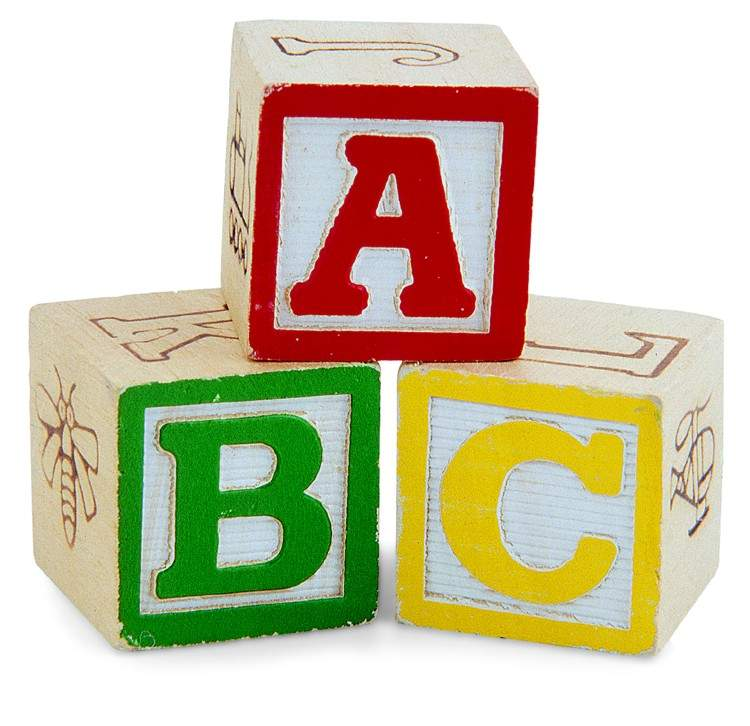
\includegraphics[width=6pc]{blocks.jpg}}\vskip 1pc\vss}

\begin{minipage}{0.3\textwidth}
\lstset{basicstyle={\fontsize{7}{7}\selectfont\ttfamily\spaceskip=3pt}}
\begin{C}
int gcd(int a, int b) {
  while (a != b) {
    if (a < b) b -= a;
    else a -= b;
  }
  return a;
}
\end{C}

%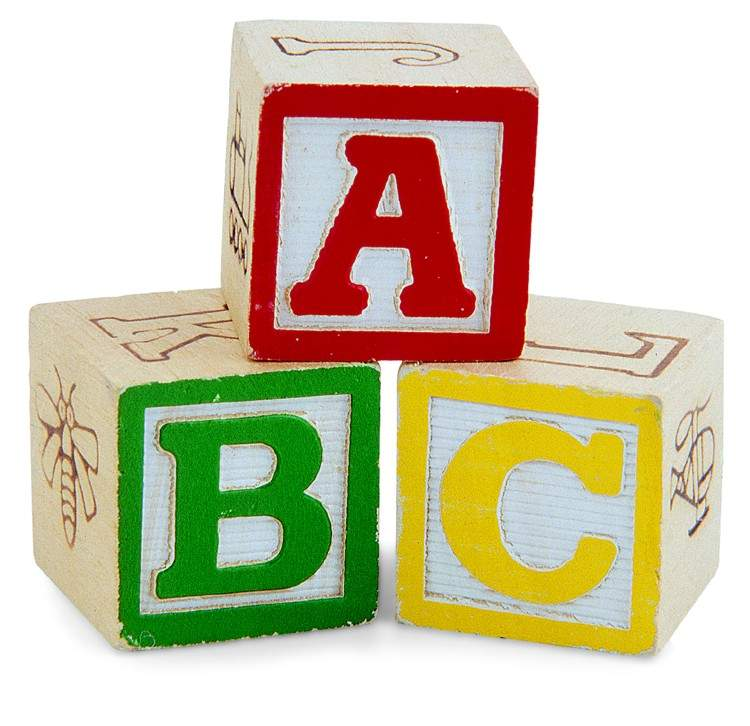
\includegraphics[width=0.8\textwidth]{blocks.jpg}
\end{minipage}
%
$\stackrel{\textrm{lower}}{\rightarrow}$
%
\begin{minipage}{0.25\textwidth}
\fontsize{8}{8}\selectfont
\begin{verbatim}
A: sne t, a, b
   bz  E, t
   slt t, a, b
   bnz B, t
   sub b, b, a
   jmp C
B: sub a, a, b
C: jmp A
E: ret a
\end{verbatim}
\end{minipage}
%
$\stackrel{\textrm{split}}{\rightarrow}$
%
\begin{minipage}{0.25\textwidth}
\fontsize{8}{8}\selectfont
\begin{verbatim}
A: sne t, a, b
   bz  E, t

   slt t, a, b
   bnz B, t

   sub b, b, a
   jmp C

B: sub a, a, b

C: jmp A

E: ret a
\end{verbatim}
\end{minipage}

The statements in a basic block all run if the first one does.

Starts with a statement following a conditional branch or is a branch target.

Usually ends with a control-transfer statement.

\end{frame}

\begin{frame}[fragile]{Control-Flow Graphs}

A CFG illustrates the flow of control among basic blocks.

\begin{columns}
  \begin{column}{0.3\textwidth}
%\fontsize{8}{8}\selectfont
\begin{verbatim}
A: sne t, a, b
   bz  E, t

   slt t, a, b
   bnz B, t

   sub b, b, a
   jmp C

B: sub a, a, b

C: jmp A

E: ret a
\end{verbatim}
  \end{column}
  \begin{column}{0.7\textwidth}
    \begin{tikzpicture}
      \matrix [nodes={font=\ttfamily,
          text width=5pc,
          draw,fill=white,drop shadow},
          column sep={4pc,between origins},
          row sep=2pc] {
        \node (entry) {A:\\sne t, a, b\\bz E, t}; &&
        \node (a1) {slt t, a, b\\bnz B, t}; &\\
        & \node (a2) {sub b, b, a\\jmp C}; &&
        \node (b) {B:\\sub a, a, b}; \\
        \node (e) {E:\\ret a}; &&
        \node (c) {C:\\jmp A}; \\
      };
      \begin{scope}[every path/.style={draw,->}]
        \path (entry.north) ++(0,2pc) -- (entry.north);
        \path (entry) -- (a1);
        \path (a1) -- (a2);
        \path (a1) -- (b);
        \path (a2) -- (c);
        \path (b) -- (c);
        \path (c) -- ++(7.5pc,0) |- ($(entry.65)+(0.5pc,1pc)$) -- (entry.65);
        \path (entry) -- (e);
      \end{scope}      
    \end{tikzpicture}
  \end{column}
\end{columns}

\end{frame}

\part{Assembly Code and Assemblers}
\frame{\partpage
\centerline{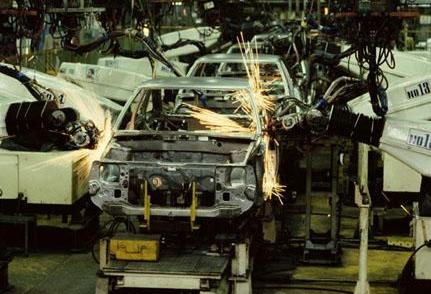
\includegraphics[width=0.5\textwidth]{assembly-line.jpg}}
}

\begin{frame}[fragile]
  \frametitle{Assembly Code}

Most compilers produce assembly code: easy to debug.

% gcc -S -O gcd.c

\begin{semiverbatim}
! gcd on the SPARC\lab{1pc}{0.5pc}{Comment}
gcd:
    cmp\lab{0.5pc}{1.5pc}{Opcode}   %o0, %o1\lab{2pc}{0.5pc}{Operand (a register)}
    be    .LL8
    nop
.LL9:\lab{1pc}{0.5pc}{Label}
    ble,a .LL2\lab{2pc}{0.5pc}{Conditional branch to a label}
    sub   %o1, %o0, %o1
    sub   %o0, %o1, %o0
.LL2:
    cmp   %o0, %o1
    bne   .LL9
    nop
.LL8:
    retl
    nop\lab{3pc}{0.5pc}{No operation}
\end{semiverbatim}

\end{frame}

\begin{frame}[fragile]
  \frametitle{Role of an Assembler}

% as -a gcd.s

Translate opcodes + operand into byte codes

\begin{semiverbatim}
              gcd: 
0000\lab{0.25pc}{2.5pc}{Address} 80A20009\lab{3.25pc}{2pc}{Instruction code}       cmp   %o0, %o1
0004 02800008       be    .LL8
0008 01000000       nop  
              .LL9:	 
000c 24800003       ble,a .LL2
0010 92224008       sub   %o1, %o0, %o1
0014 90220009       sub   %o0, %o1, %o0
              .LL2:	 
0018 80A20009       cmp   %o0, %o1
001c 12BFFFFC       bne   .LL9
0020 01000000       nop
              .LL8:
0024 81C3E008       retl
0028 01000000       nop
\end{semiverbatim}

\end{frame}

\begin{frame}[fragile]
  \frametitle{Encoding Example}

\begin{verbatim}
sub   %o1, %o0, %o1
\end{verbatim}

Encoding of ``SUB'' on the SPARC:

\begin{tabular}{|*{7}{c|}}
\hline
10 & rd & 000100 & rs1 & 0 & reserved & rs2 \\
\hline
\multicolumn{1}{l}{31} &
\multicolumn{1}{l}{29} &
\multicolumn{1}{l}{24} &
\multicolumn{1}{l}{18} &
\multicolumn{1}{l}{13} &
\multicolumn{1}{l}{12} &
\multicolumn{1}{l}{4} \\
\end{tabular}

rd  = \%o1 = 01001

rs1 = \%o1 = 01001

rs2 = \%o0 = 00100


10 01001 000100 01001 0 00000000 01000 \\
1001 0010 0010 0010 0100 0000 0000 1000

= 0x92228004

\end{frame}

\begin{frame}[fragile]
  \frametitle{Role of an Assembler}

Transforming symbolic addresses to concrete ones.

Example: Calculating PC-relative branch offsets.

\vspace{2pc}

\begin{semiverbatim}
000c 24800003\lab{1pc}{2pc}{LL2 is 3 words away}       ble,a .LL2
0010 92224008       sub   %o1, %o0, %o1
0014 90220009       sub   %o0, %o1, %o0
              .LL2:	 
0018 80A20009       cmp   %o0, %o1
\end{semiverbatim}

\end{frame}

\begin{frame}[fragile]
  \frametitle{Role of an Assembler}

Most assemblers are ``two-pass'' because they can't calculate
everything in a single pass through the code.

\vspace{2pc}

\begin{semiverbatim}
             .LL9:
000c 24800003     ble,a .LL2\lab{1pc}{2pc}{Don't know offset of LL2}
0010 92224008     sub   %o1, %o0, %o1
0014 90220009     sub   %o0, %o1, %o0
             .LL2:	 
0018 80A20009     cmp   %o0, %o1
001c 12BFFFFC     bne   .LL9\lab{1pc}{0pc}{Know offset of LL9}

\end{semiverbatim}

\end{frame}

\begin{frame}[fragile]
  \frametitle{Role of an Assembler}

Constant data needs to be aligned.

\begin{C}
char a[] = "Hello";
int b[3] = { 5, 6, 7 };
\end{C}

\begin{minipage}{\textwidth}
\fontsize{8}{8}\selectfont
\begin{semiverbatim}
                .section\lab{2pc}{2.5pc}{Assembler directive} ".data"   \hlt{\texttt{! ``This is data''}}
                .global a          \hlt{\texttt{! ``Let other files see a}}
                .type   a,#object  \hlt{\texttt{! ``a is a variable''}}
                .size   a,6        \hlt{\texttt{! ``six bytes long''}}
             a:
0000 48656C6C   .asciz  "Hello"    \hlt{\texttt{! zero-terminated ASCII}}
     6F00      

                .global b
0006 0000\lab{1.5pc}{2pc}{Bytes added to ensure alignment}       \hlt{.align 4}
                .type   b,#object
                .size   b,12
             b:
0008 00000005   .uaword 5
000c 00000006   .uaword 6
0010 00000007   .uaword 7
\end{semiverbatim}
\end{minipage}

\end{frame}

\begin{frame}[fragile]
  \frametitle{Role of an Assembler}

The MIPS has pseudoinstructions:

``Load the immediate value 0x12345abc into register 14:''

\begin{verbatim}
li $14, 0x12345abc
\end{verbatim}

expands to

\begin{verbatim}
lui $14, 0x1234
ori $14, 0x5abc
\end{verbatim}

``Load the upper 16 bits, then OR in the lower 16''

MIPS instructions have 16-bit immediate values at most

RISC philosophy: small instructions for common case

\end{frame}

\part{Optimization: Register Allocation}
\frame{\partpage
\centerline{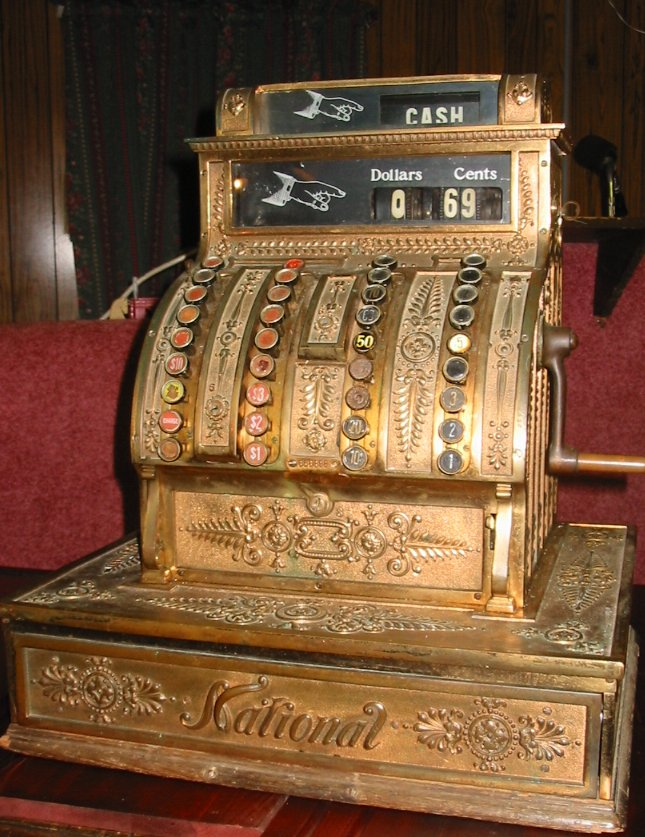
\includegraphics[width=0.4\textwidth]{national-cash-register.jpg}}
}

\begin{frame}[fragile]{Optimization: Register Allocation}

Where to put temporary results?  The easiest is to put everything on the stack.

\begin{C}
int bar(int g, int h, int i,
        int j, int k, int l)
{
  int a, b, c, d, e, f;
  a = foo(g);
  b = foo(h);
  c = foo(i);
  d = foo(j);
  e = foo(k);
  f = foo(l);
  return a + b + c + d + e + f;
}
\end{C}

\end{frame}

\begin{frame}[fragile]
  \frametitlelogo{Quick Review of the x86 Architecture}{0.25\textwidth}{80386.jpg}

Eight ``general-purpose'' 32-bit registers:

eax
ebx
ecx
edx
ebp
esi
edi
esp

esp is the stack pointer

ebp is the base (frame) pointer

\begin{semiverbatim}
addl %eax, %edx \hlt{\textrm{eax + edx \(\rightarrow\) edx}}
\end{semiverbatim}

Base-pointer-relative addressing:

\begin{semiverbatim}
movl 20(%ebp), %eax \hlt{\textrm{Load word at ebp+20 into eax}}
\end{semiverbatim}



\end{frame}

\newsavebox{\callbox}
\begin{lrbox}{\callbox}
\lstset{basicstyle={\fontsize{7}{7}\selectfont\ttfamily\spaceskip=3pt}}
\begin{C}
int bar(int g, int h, int i,
        int j, int k, int l)
{
  int a, b, c, d, e, f;
  a = foo(g);
  b = foo(h);
  c = foo(i);
  d = foo(j);
  e = foo(k);
  f = foo(l);
  return a + b + c + d + e + f;
}
\end{C}
\end{lrbox}


\begin{frame}[fragile]
  \frametitle{Unoptimized GCC on the x86}

\begin{columns}
  \begin{column}{0.65\textwidth}
\fontsize{9}{9}\selectfont
\begin{semiverbatim}
movl 24(%ebp),%eax  \hlt{\textrm{% Get k}}
pushl %eax          \hlt{\textrm{% Push argument}} 
call foo            \hlt{\textrm{% e = foo(k);}} 
addl $4,%esp        \hlt{\textrm{% Make room for e}} 
movl %eax,%eax      \hlt{\textrm{% Does nothing}} 
movl %eax,-20(%ebp) \hlt{\textrm{% Save return value on stack}} 

movl 28(%ebp),%eax  \hlt{\textrm{% Get l}}                      
pushl %eax          \hlt{\textrm{% Push argument}}        
call foo            \hlt{\textrm{% f = foo(l);}}                
addl $4,%esp        \hlt{\textrm{% Make room for f}} 
movl %eax,%eax      \hlt{\textrm{% Does nothing}}               
movl %eax,-24(%ebp) \hlt{\textrm{% Save return value on stack}} 

movl -20(%ebp),%eax \hlt{\textrm{% Get f}}
movl -24(%ebp),%edx \hlt{\textrm{% Get e}}
addl %edx,%eax      \hlt{\textrm{% e + f}}
movl %eax,%edx      \hlt{\textrm{% Accumulate in edx}}
addl -16(%ebp),%edx \hlt{\textrm{% d + (e+f)}}
movl %edx,%eax      \hlt{\textrm{% Accumulate in edx}}
\end{semiverbatim}
  \end{column}
  \begin{column}{0.45\textwidth}
    \usebox{\callbox}
  \end{column}
\end{columns}
\end{frame}

\begin{frame}[fragile]{Optimized GCC on the x86}
\begin{columns}
  \begin{column}{0.65\textwidth}
\fontsize{9}{9}\selectfont
\begin{semiverbatim}
movl 20(%ebp),%edx  \hlt{\textrm{% Get j}}
pushl %edx          \hlt{\textrm{% Push argument}}
call foo            \hlt{\textrm{% d = foo(j);}} 
movl %eax,%esi      \hlt{\textrm{% save d in esi}}

movl 24(%ebp),%edx  \hlt{\textrm{% Get k}}
pushl %edx          \hlt{\textrm{% Push argument}}
call foo            \hlt{\textrm{% e = foo(k);}} 
movl %eax,%ebx      \hlt{\textrm{% save e in ebx}}

movl 28(%ebp),%edx  \hlt{\textrm{% Get l}}
pushl %edx          \hlt{\textrm{% Push argument}}
call foo            \hlt{\textrm{% f = foo(l);}}

addl %ebx,%eax      \hlt{\textrm{% e + f}}
addl %esi,%eax      \hlt{\textrm{% d + (e+f)}}
\end{semiverbatim}
  \end{column}
  \begin{column}{0.45\textwidth}
    \usebox{\callbox}
  \end{column}
\end{columns}
\end{frame}

\begin{frame}[fragile]
  \frametitle{Unoptimized vs. Optimized}
\begin{columns}
  \begin{column}[t]{0.2\textwidth}
\fontsize{9}{9}\selectfont
\begin{semiverbatim}





movl 24(%ebp),%eax 
pushl %eax         
call foo           
addl $4,%esp       
movl %eax,%eax     
movl %eax,-20(%ebp)
		   
movl 28(%ebp),%eax 
pushl %eax         
call foo           
addl $4,%esp       
movl %eax,%eax     
movl %eax,-24(%ebp)
		   
movl -20(%ebp),%eax
movl -24(%ebp),%edx
addl %edx,%eax     
movl %eax,%edx     
addl -16(%ebp),%edx
movl %edx,%eax    
\end{semiverbatim}
  \end{column}
  \begin{column}[t]{0.2\textwidth}
\fontsize{9}{9}\selectfont
\begin{semiverbatim}
movl 20(%ebp),%edx
pushl %edx        
call foo          
movl %eax,%esi    
		  
movl 24(%ebp),%edx
pushl %edx        
call foo          
movl %eax,%ebx    


		  
movl 28(%ebp),%edx
pushl %edx        
call foo          





		  
addl %ebx,%eax    

addl %esi,%eax    
\end{semiverbatim}
  \end{column}
  \begin{column}[t]{0.3\textwidth}
    \vspace{5pc}
    \usebox{\callbox}
  \end{column}
\end{columns}

\end{frame}

\part{Separate Compilation and Linking}
\frame{\partpage}

\begin{frame}{Separate Compilation and Linking}

\begin{tikzpicture}
  \node {foo} [grow'=up,<-,level distance=5pc,sibling distance=5pc,
    line width=2pt]
  child {node {foo.o}
    child {node {foo.s}
      child {node{foo.c}
       edge from parent [red] node [left] {Compiler}}
     edge from parent [blue] node [left] {Assembler}}
    edge from parent node [left,anchor=north east] {Linker}
  }
  child {node {bar.o}
    child {node {bar.s}
      child {node {bar.c}
       edge from parent [red] node [right] {cc}}
    edge from parent [blue] node [right] {as}}
  }
  child [missing]
  child {node {libc.a}
    child {node {printf.o}
      edge from parent [darkgreen] node [left,anchor=north east] {Archiver}}
    child {node {fopen.o}
      edge from parent [darkgreen]
    }
    child {node {malloc.o}
      edge from parent [darkgreen] node [right,anchor=north west] {ar}
    }
    edge from parent node [right,anchor=north west] {ld}
  }  
  ;
\end{tikzpicture}

\end{frame}

\begin{frame}[fragile]
  \frametitlelogo{Linking}{0.23\textwidth}{chain.jpg}

Goal of the linker is to combine the disparate \\
pieces of the program into a coherent whole.

\vspace{1pc}

\def\{{\char`\{}
\def\}{\char`\}}

\footnotesize
\begin{columns}
  \begin{column}[t]{0.33\textwidth}
\hlt{file1.c:}
\begin{semiverbatim}
#include <stdio.h>
char \rnode{a1}{a}[] = "Hello";
extern void \rnode{bar1}{bar}();

int main() \{
  \rnode{bar11}{bar}();
\}

void \rnode{baz1}{baz}(char *s) \{
  \rnode{printf1}{printf}("%s", s);
\}
\end{semiverbatim}
  \end{column}
  \begin{column}[t]{0.33\textwidth}
\hlt{file2.c:}
\begin{semiverbatim}
#include <stdio.h>
extern char \rnode{a2}{a}[];
extern void \rnode{baz3}{baz}(char *);

static char b[6];

void \rnode{bar2}{bar}() \{
  \rnode{strcpy2}{strcpy}(b, \rnode{a21}{a});
  \rnode{baz2}{baz}(b);
\}
\end{semiverbatim}
  \end{column}
  \begin{column}[t]{0.33\textwidth}
\hlt{libc.a:}
\begin{semiverbatim}
int
\rnode{printf3}{printf}(char *s, ...)
\{
  /* ... */
\}

char *
\rnode{strcpy3}{strcpy}(char *d,
       char *s)
\{
  /* ... */
\}
\end{semiverbatim}
  \end{column}
\end{columns}

\pause

\begin{tikzpicture}[connecting lines]
    \draw (a2) to [bend right] (a1);
    \draw (a21) to [bend right] (a1);
    \draw (bar1) to [bend left] (bar2);
    \draw (bar11) to [bend left] (bar2);
    \draw (baz2) to [bend right] (baz1);
    \draw (baz3) to [bend right] (baz1);
    \draw (printf1) to [bend right] (printf3);
    \draw (strcpy2) to [bend right] (strcpy3);
\end{tikzpicture}

\end{frame}

\begin{frame}
  \frametitle{Linking}

\begin{columns}
  \begin{column}{0.25\textwidth}
\begin{tabular}{c}
file1.o \\
\framednode{a1}{a=``Hello''} \\
\framednode{main1}{main()} \\
\framednode{baz1}{baz()} \\
\end{tabular}
  \end{column}
  \begin{column}{0.25\textwidth}
\onslide<2>{
\begin{tabular}{c}
a.out \\
.text segment \\
\framebox{
 \begin{tabular}{c}
 \framednode{main}{main()} \\
 \framednode{baz}{baz()} \\
 \framednode{bar}{bar()}
 \end{tabular}
}
\\
.data segment \\
\framebox{
  \framednode{a}{a=``Hello''}
}
\\
.bss segment \\
\framebox{
  \framednode{b}{char b[6]}
}
\end{tabular}
}
  \end{column}
  \begin{column}{0.25\textwidth}
\begin{tabular}{c}
file2.o \\
\framednode{b2}{char b[6]} \\
\framednode{bar2}{bar()} \\
\end{tabular}
\only<2>{
\begin{tikzpicture}[connecting lines]
    \draw (a1.east) to (a.west);
    \draw (main1.east) to (main.west);
    \draw (baz1.east) to (baz.west);
    \draw (b2.west) to (b.east);
    \draw (bar2.west) to (bar.east);
\end{tikzpicture}
}
  \end{column}
  \begin{column}{0.3\textwidth}
\onslide<2>{
\begin{center}
\textcolor{red}{.text}

Code of program

\medskip

\textcolor{red}{.data}

Initialized data

\medskip

\textcolor{red}{.bss}

Uninitialized data

``Block Started by Symbol''
\end{center}
}
  \end{column}
\end{columns}

\end{frame}

\begin{frame}
  \frametitle{Object Files}
Relocatable: Many need to be pasted together.  Final in-memory address
of code not known when program is compiled

Object files contain

\begin{itemize}
\item imported symbols (unresolved ``external'' symbols)

\item relocation information (what needs to change)

\item exported symbols (what other files may refer to)
\end{itemize}

\end{frame}

\begin{frame}[fragile]
  \frametitle{Object Files}

\def\{{\char`\{}
\def\}{\char`\}}

\footnotesize
\begin{minipage}[t]{0.5\textwidth}
\hlt{file1.c:}
\begin{semiverbatim}
#include <stdio.h>
char \rnode{a1}{a}[] = "Hello";
extern void \rnode{bar1}{bar}();

int main() \{
  \rnode{bar11}{bar}();
\}

void \rnode{baz1}{baz}(char *s) \{
  \rnode{printf1}{printf}("%s", s);
\}
\end{semiverbatim}
\end{minipage}
\begin{minipage}[t]{0.4\textwidth}
\vspace{1pc}

\rnode{export}{e}xported symbols
\vspace{4pc}

\rnode{import}{i}mported symbols
\end{minipage}

\begin{tikzpicture}[connecting lines]
  \draw (import) to (bar11);
  \draw (import) to (printf1);
  \draw (export) to (main1);
  \draw (export) to (baz1);
  \draw (export) to (a1);
\end{tikzpicture}

\end{frame}

\begin{frame}[fragile]{Object Files}

\begin{columns}
  \begin{column}{0.3\textwidth}
\hlt{file1.c:}

\begin{C}
#include <stdio.h>
char a[] = "Hello";
extern void bar();

int main() {
  bar();
}

void baz(char *s) {
  printf("%s", s);
}
\end{C}
  \end{column}
  \begin{column}{0.7\textwidth}
\fontsize{10}{10}\selectfont
\begin{verbatim}
# objdump -x file1.o
Sections:
Idx Name    Size VMA LMA Offset Algn
  0 .text   038  0   0   034    2**2
  1 .data   008  0   0   070    2**3
  2 .bss    000  0   0   078    2**0
  3 .rodata 008  0   0   078    2**3

SYMBOL TABLE:
0000 g O .data   006 a
0000 g F .text   014 main
0000     *UND*   000 bar
0014 g F .text   024 baz
0000     *UND*   000 printf

RELOCATION RECORDS FOR [.text]:
OFFSET   TYPE          VALUE 
0004 R_SPARC_WDISP30   bar
001c R_SPARC_HI22      .rodata
0020 R_SPARC_LO10      .rodata
0028 R_SPARC_WDISP30   printf
\end{verbatim}
  \end{column}
\end{columns}

\end{frame}

\begin{frame}[fragile]{Object Files}


\begin{columns}
  \begin{column}{0.3\textwidth}
\hlt{file1.c:}

\begin{C}
#include <stdio.h>
char a[] = "Hello";
extern void bar();

int main() {
  bar();
}

void baz(char *s) {
  printf("%s", s);
}
\end{C}
  \end{column}
  \begin{column}{0.7\textwidth}
\fontsize{10}{10}\selectfont
\begin{semiverbatim}
# objdump -d file1.o
0000 <main>:
 0: 9d e3 bf 90 save  %sp, -112, %sp
 4: 40 00 00 00 call  4 <main+0x4>
    \hlt{4: R_SPARC_WDISP30 bar}
 8: 01 00 00 00 nop 
 c: 81 c7 e0 08 ret 
10: 81 e8 00 00 restore 
	       
0014 <baz>:    
14: 9d e3 bf 90 save  %sp, -112, %sp
18: f0 27 a0 44 st  %i0, [ %fp + 0x44 ]
1c: 11 00 00 00 sethi  %hi(0), %o0
    \hlt{1c: R_SPARC_HI22 .rodata}
20: 90 12 20 00 mov  %o0, %o0
    \hlt{20: R_SPARC_LO10 .rodata}
24: d2 07 a0 44 ld  [ %fp + 0x44 ], %o1
28: 40 00 00 00 call  28 <baz+0x14>
    \hlt{28: R_SPARC_WDISP30 printf}
2c: 01 00 00 00 nop 
30: 81 c7 e0 08 ret 
34: 81 e8 00 00 restore
\end{semiverbatim}
  \end{column}
\end{columns}

\end{frame}

\begin{frame}[fragile]
  \frametitle{Before and After Linking}

\begin{columns}
  \begin{column}{0.3\textwidth}
\begin{C}
int main() {
  bar();
}

void baz(char *s) {
  printf("%s", s);
}
\end{C}
  \end{column}
  \begin{column}{0.7\textwidth}
\begin{itemize}

\item Combine object files

\item Relocate each function's code

\item Resolve previously unresolved symbols

\end{itemize}
  \end{column}
\end{columns}

\begin{columns}
  \begin{column}{0.5\textwidth}
\fontsize{7}{7}\selectfont
\begin{semiverbatim}
0000 <main>:
 0: 9d e3 bf 90 save  %sp, -112, %sp
 4: 40 00 00 00 call  4 <main+0x4>
    \hlt{4: R_SPARC_WDISP30 bar}
 8: 01 00 00 00 nop 
 c: 81 c7 e0 08 ret 
10: 81 e8 00 00 restore 

0014 <baz>:    
14: 9d e3 bf 90 save  %sp, -112, %sp
18: f0 27 a0 44 st  %i0, [ %fp + 0x44 ]
1c: 11 00 00 00 sethi  %hi(0), %o0
    \hlt{1c: R_SPARC_HI22 .rodata}\lab{4pt}{0pc}{Unresolved symbol}
20: 90 12 20 00 mov  %o0, %o0
    \hlt{20: R_SPARC_LO10 .rodata}
24: d2 07 a0 44 ld  [ %fp + 0x44 ], %o1
28: 40 00 00 00 call  28 <baz+0x14>
    \hlt{28: R_SPARC_WDISP30 printf}
2c: 01 00 00 00 nop 
30: 81 c7 e0 08 ret 
34: 81 e8 00 00 restore
\end{semiverbatim}
  \end{column}
  \begin{column}{0.5\textwidth}
\fontsize{7}{7}\selectfont
\begin{semiverbatim}
105f8\lab{2pt}{1.5pc}{Code starting address changed} <main>:
105f8: 9d e3 bf 90 save %sp, -112, %sp
\hlt{105fc: 40 00 00 0d call 10630 <bar>}

10600: 01 00 00 00 nop 
10604: 81 c7 e0 08 ret 
10608: 81 e8 00 00 restore 
		  
1060c <baz>:	  
1060c: 9d e3 bf 90 save  %sp, -112, %sp
10610: f0 27 a0 44 st    %i0, [ %fp + 0x44 ]
\hlt{10614: 11 00 00 41 sethi %hi(0x10400), %o0}

\hlt{10618: 90 12 23 00 or    %o0, 0x300, %o0}

1061c: d2 07 a0 44 ld    [ %fp + 0x44 ], %o1
\hlt{10620: 40 00 40 62 call  207a8}

10624: 01 00 00 00 nop 
10628: 81 c7 e0 08 ret 
1062c: 81 e8 00 00 restore 
\end{semiverbatim}
  \end{column}
\end{columns}

\end{frame}


\begin{frame}[fragile]
  \frametitle{Linking Resolves Symbols}

\begin{minipage}[t]{0.4\textwidth}
\hlt{file1.c:}

\begin{C}
#include <stdio.h>
char a[] = "Hello";
extern void bar();

int main() {
  bar();
}

void baz(char *s) {
  printf("%s", s);
}
\end{C}

\hlt{file2.c:}

\begin{C}
#include <stdio.h>
extern char a[];
extern void baz(char *);

static char b[6];

void bar() {
  strcpy(b, a);
  baz(b);
}
\end{C}
\end{minipage}
\begin{minipage}[t]{0.28\textwidth}
\fontsize{7}{7}\selectfont
\begin{semiverbatim}
105f8 <main>:
105f8: 9d e3 bf 90 save %sp, -112, %sp
\hlt{105fc: 40 00 00 0d call 10630 <bar>}
10600: 01 00 00 00 nop 
10604: 81 c7 e0 08 ret 
10608: 81 e8 00 00 restore 
		  
1060c <baz>:	  
1060c: 9d e3 bf 90 save  %sp, -112, %sp
10610: f0 27 a0 44 st    %i0, [ %fp + 0x44 ]
\hlt{10614: 11 00 00 41 sethi %hi(0x10400), %o0}
\hlt{10618: 90 12 23 00 or    %o0, 0x300, %o0   ! "%s"}
1061c: d2 07 a0 44 ld    [ %fp + 0x44 ], %o1
\hlt{10620: 40 00 40 62 call  207a8             ! printf}
10624: 01 00 00 00 nop 
10628: 81 c7 e0 08 ret 
1062c: 81 e8 00 00 restore 
		  
10630 <bar>:	  
10630: 9d e3 bf 90 save  %sp, -112, %sp
\hlt{10634: 11 00 00 82 sethi %hi(0x20800), %o0
10638: 90 12 20 a8 or    %o0, 0xa8, %o0    ! 208a8 <b>
1063c: 13 00 00 81 sethi %hi(0x20400), %o1
10640: 92 12 63 18 or    %o1, 0x318, %o1   ! 20718 <a>}
\hlt{10644: 40 00 40 4d call  20778             ! strcpy}
10648: 01 00 00 00 nop 
\hlt{1064c: 11 00 00 82 sethi %hi(0x20800), %o0
10650: 90 12 20 a8 or    %o0, 0xa8, %o0    ! 208a8 <b>
10654: 7f ff ff ee call  1060c <baz>}
10658: 01 00 00 00 nop 
1065c: 81 c7 e0 08 ret 
10660: 81 e8 00 00 restore 
10664: 81 c3 e0 08 retl 
10668: ae 03 c0 17 add  %o7, %l7, %l7
\end{semiverbatim}
\end{minipage}

\end{frame}

\end{document}

% Local Variables:
% mode: latex
% compile-command: "make codegen.pdf"
% End:

